%*******************************************************************************************%
%				A CONTRIBUTION ON THE MODULAR MODELLING OF MULTIBODY SYSTEMS				%
% 																					   		%
% June 2015															 						%
% Author: Renato Maia Matarazzo Orsino														%
% bash modularmodelling.sh					 												%
% 																							%
%*******************************************************************************************%


\documentclass[25pt,landscape]{beamer}
	\mode<presentation> {
	  \usetheme{Warsaw}
	  \setbeamercovered{transparent}
	  \useoutertheme{shadow}
	  \useoutertheme{infolines}
	  \useinnertheme{rounded}
	  \setbeamertemplate{theorems}[numbered]
	  \setbeamertemplate{bibliography item}[text]
	  \usecolortheme{default}
	}


% - INPUT - %
\usepackage[T1]{fontenc}
\usepackage[latin1]{inputenc}


% - MATH - %
\usepackage{amsmath,amsfonts,amssymb}
\usepackage{amsthm}
\usepackage{accents}


% - GENERAL - %
\usepackage{cmbright}
\usepackage{natbib}
\usepackage{color}
% \usepackage[pdftex,dvipsnames]{color}
% \usepackage{geometry}
\usepackage{array,hhline,supertabular,tabularx}
\usepackage{hyperref}
% \usepackage[colorlinks,citecolor=black,urlcolor=black,linkcolor=black]{hyperref}
\usepackage{graphicx}
% \usepackage[pdftex]{graphicx}
\usepackage{enumitem}
\usepackage{float}
\usepackage{titlesec}
\usepackage{pp4link}
\usepackage{mpmulti}
\usepackage{multimedia}
\usepackage[display]{texpower}
\usepackage{multicol}
\usepackage[overlay,absolute]{textpos}
\setlength{\TPHorizModule}{1cm}
\setlength{\TPVertModule}{1cm}
\usepackage{multicol}

% - SPECIAL - %
\usepackage{EXTRAS/special-char}
\usepackage{EXTRAS/special-conf}




%---------------------------------------------------------------------------------------%
%										BEAMER											%
%---------------------------------------------------------------------------------------%

\begin{document}


\begin{frame}
    \titlepage
\end{frame}



%--- INTRODU\c{c}\~aO -------------------------------------------------------------------------%


%\begin{frame}{Test frame}
%    \begin{textblock}{12}(0.4,1.5)
%            \begin{exampleblock}{Answered Questions}
%            \end{exampleblock}
%            \begin{block}{Defini\c{c}\~ao}
%                A \alert{set} consists of elements.
%            \end{block}
%    \end{textblock}
%\end{frame}

\begin{frame}{Sistema de interesse}
    \begin{figure}[H]
		\centering
		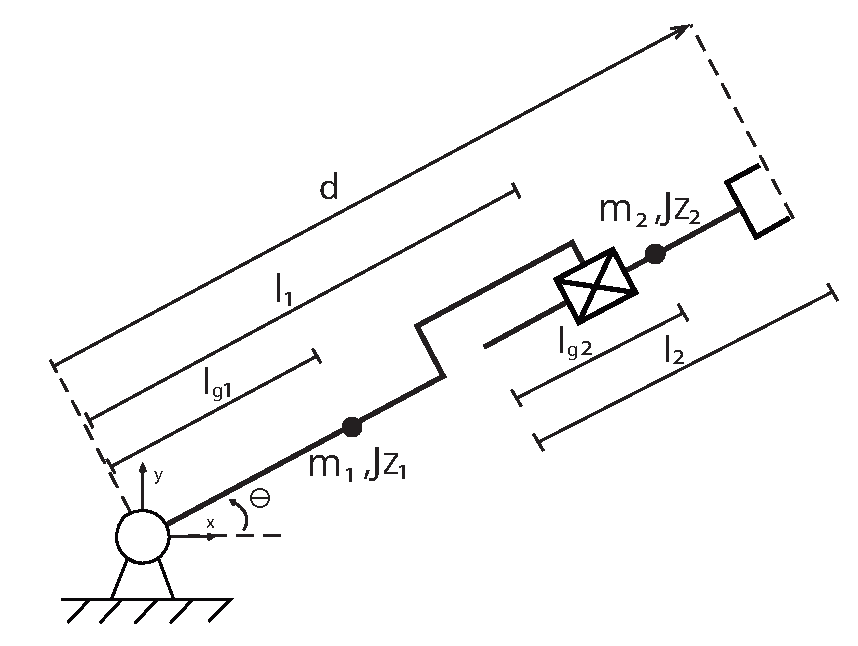
\includegraphics[scale=0.5]{FIGURES/RP.pdf}  
		\caption{Mecanismo RP}
		\label{fig:1}
	\end{figure}
\end{frame}

\begin{frame}{Equa\c{c}\~oes din\^amicas}
    \begin{block}{}
        \begin{equation}
			\mH(\mq) \ddot{\mq} + \mh(\mq, \dot{\mq}) = \mtau
		\end{equation}
		Sendo:
		\begin{equation}
			\mq = \begin{bmatrix} \theta & d \end{bmatrix}^\msT
		\end{equation}

		\begin{equation}
			\mH(\mq) = 
			\begin{bmatrix}
				Jz_1 + Jz_2 + m_1 lg_1^2 + m_2 (d - l_2 + l_{g2})^2 & 0 \\
				0 & m_2
			\end{bmatrix}
		\end{equation}

		\begin{equation}
			\mh(\mq, \dot{\mq}) = 
			\begin{bmatrix}
				2 m_2 (d-l_2+l_{g2}) \dot{\theta} \dot{d} - (m_1 l_{g1} + m_2 (d-l_2 + l_{g2}) ) g \,\ccos \theta \\
				-m_2  (d-l_2+l_{g2})\dot{\theta}^2  - m_2 g \, \ssin \theta
			\end{bmatrix}
		\end{equation}		
    \end{block}
\end{frame}

\begin{frame}{Lei de Controle}
    \begin{block}{Feedback Linearization}
		\begin{equation}
			\mtau = \mh(\mq,\dot{\mq}) + \mH(\mq) ( \ddot{\mq} + k_v \dot{\me} + k_p \me ) 
		\end{equation}
    \end{block}
\end{frame}

\begin{frame}{Espaço de estados n\~ao linear}
    \begin{block}{}
        \begin{equation}
        	\mx = \begin{bmatrix} \dot{\mq}^\msT & \mq^\msT \end{bmatrix}^\msT
        \end{equation}

        \begin{equation}
        	\begin{cases}
        		\dot{\mx} =
        		\begin{bmatrix} 
        			\mH^\msI(\mtau - \mh) \\
        			\dot{\mq}
        		\end{bmatrix} \\
        		\my = \mq
        	\end{cases}
        \end{equation}
    \end{block}
\end{frame}

\begin{frame}{Equa\c{c}\~oes din\^amicas linearizadas}
    \begin{block}{}
		\begin{equation}
			\mf(\mq, \dot{\mq}, \ddot{\mq}, \mtau) = \mH(\mq) \ddot{\mq} + \mh(\mq, \dot{\mq}) - \mtau = \mzr
		\end{equation}

		\begin{equation}
			\mf(\mq, \dot{\mq}, \ddot{\mq}, \mtau) \approx  \mf^* + \frac{\partial \mf}{\partial \mq}^* \Delta \mq + \frac{\partial \mf}{\partial \dot{\mq}}^* \Delta \dot{\mq} + \frac{\partial \mf}{\partial \ddot{\mq}}^* \Delta \ddot{\mq} + \frac{\partial \mf}{\partial \mtau}^* \Delta \mtau
		\end{equation}
    \end{block}
\end{frame}

\begin{frame}{Equa\c{c}\~oes din\^amicas linearizadas}
    \begin{block}{}
    	\begin{equation} \label{eq:M}
			\mM(\mq^*) = \frac{\partial \mf}{\partial \ddot{\mq}}^*  = \mH^*
		\end{equation}
		\begin{equation} \label{eq:V}
			\mV(\mq^*, \dot{\mq}^*) =\frac{\partial \mf}{\partial \dot{\mq}}^* =  \frac{\partial \mh}{\partial \dot{\mq}}^*
		\end{equation}
		\begin{equation} \label{eq:G}
			\mG(\mq^*) = \frac{\partial \mf}{\partial \mq}^* = \Big( \frac{\partial (\mH \cdot \ddot{\mq})}{\partial \mq} + \frac{\partial \mh}{\partial \mq} \Big)^*
		\end{equation}
		\begin{equation}
			\frac{\partial \mf}{\partial \mtau}^* = -\mone
		\end{equation}
    \end{block}
\end{frame}

\begin{frame}{Equa\c{c}\~oes din\^amicas linearizadas}
    \begin{block}{}
    	\begin{equation}
			\mM(\mq^*) = 
			\begin{bmatrix}
				Jz_1 + Jz_2 + m_1 lg_1^2 + m_2 (d^* - l_2 + l_{g2})^2 & 0 \\
				0 & m_2
			\end{bmatrix}
		\end{equation}

		\begin{equation}
			\mV(\mq^*, \dot{\mq}^*) =
			\begin{bmatrix}
				2 m_2 (d^* -l_2+l_{g2}) \dot{d}^* & 2 m_2 (d^* -l_2+l_{g2}) \dot{\theta}^* \\
				-2 m_2 (d^* -l_2+l_{g2}) \dot{\theta}^* & 0
			\end{bmatrix}
		\end{equation}

		\footnotesize
		\begin{equation}
			\mG(\mq^*) =
			\begin{bmatrix}
				\big( m_1 l_{g1}  + m_2 ( d^* -l_2 + l_{g2})\big) g \,\ssin \theta^* & m_2 \left(2 \dot{d}^* \dot{\theta}^*+2  (d^*-l_2+l_{g2})\ddot{\theta}^* -g \, \ccos \theta^*\right) \\
				-m_2 g \, \ccos\theta^* & -m_2 (\dot{\theta}^*)^2
			\end{bmatrix}
		\end{equation}
		\normalsize
    \end{block}
\end{frame}

\begin{frame}{Equa\c{c}\~oes din\^amicas linearizadas}
    \begin{block}{}
		\begin{equation} \label{eq:SisLinSS}
			\begin{cases}
				\begin{bmatrix}
					\Delta\ddot{\mq} \\
					\Delta\dot{\mq} \\
				\end{bmatrix}
				=
				\begin{bmatrix}
					-\mM^{-1} \mV& -\mM^{-1} \mG \\
					\mone & \mzr
				\end{bmatrix}
				\begin{bmatrix}
					\Delta\dot{\mq} \\
					\Delta\mq \\
				\end{bmatrix}
				+
				\begin{bmatrix}
					\mM^{-1} \\
					\mzr
				\end{bmatrix} \Delta\mtau
				\\
				\Delta\my = \begin{bmatrix}
					\mzr & \mone
					\end{bmatrix}
				\begin{bmatrix}
					\Delta\dot{\mq} \\
					\Delta\mq \\
				\end{bmatrix}
			\end{cases}
		\end{equation}
    \end{block}
\end{frame}

\begin{frame}{Equa\c{c}\~oes din\^amicas linearizadas}
    \begin{block}{}
		\begin{equation}
			\begin{cases}
				\Delta\dot{\mx} = \mA \cdot \Delta\mx + \mB \cdot \Delta\mtau \\
				\Delta\my = \mC \cdot \Delta\mx
			\end{cases}
		\end{equation}
		
		
		\begin{equation}
			\mA = \begin{bmatrix}
			-\mM^{-1} \mV& -\mM^{-1} \mG \\
			\mone & \mzr
			\end{bmatrix}
		\end{equation}
		\begin{equation}
			\mB = \begin{bmatrix}
			\mM^{-1} \\
			\mzr
			\end{bmatrix}
		\end{equation}
		\begin{equation}
			\mC = \begin{bmatrix}
			\mzr & \mone
			\end{bmatrix}
		\end{equation}
    \end{block}
\end{frame}

\begin{frame}{Discretiza\c{c}\~ao do Sistema}
    \begin{block}{Hipótese}
		O esfor\c{c}o de controle permanece constante durante cada passo de integra\c{c}\~ao
    \end{block}
\end{frame}

\begin{frame}{Discretiza\c{c}\~ao do Sistema}
	\framesubtitle{RK4}
    \begin{block}{}
		\begin{equation}
			\begin{align*}
				\dot{x} &=  f(t, x), \; x(t_0) = x_0 \\
				\\
				x_{k+1} &=  x_k + \frac{T}{6} \Big( k_1 + 2 k_2 + 2 k_3 + k_4 \Big) = g(t_k, x_k) \\
				t_{k+1} &=  t_k + T \\
				\\
				k_1 &=  f(t_k, x_k) \\
				k_2 &=  f \Big( t_k + \frac{T}{2}, x_k + \frac{T}{2} k_1 \Big) \\
				k_3 &=  f \Big( t_k + \frac{T}{2}, x_k + \frac{T}{2} k_2 \Big) \\
				k_4 &=  f(t_k + T, x_k + T k_3) \\
			\end{align*}
		\end{equation}
    \end{block}
\end{frame}

\begin{frame}{Discretiza\c{c}\~ao do Sistema}
	\framesubtitle{Jacobiano do RK4}
    \begin{block}{}
    	\begin{equation}
    		A = \frac{\partial f}{\partial x}
    	\end{equation}

		\begin{equation}
			\phi = \frac{\partial g}{\partial x_k} = 1 + \frac{T}{6} \Big( \frac{\partial k_1}{\partial x_k} + 2 \frac{\partial k_2}{\partial x_k}  + 2 \frac{\partial k_3}{\partial x_k}  + \frac{\partial k_4}{\partial x_k}  \Big)
		\end{equation}
		\begin{equation}
			\frac{\partial k_1}{\partial x_k}  =  \frac{\partial f}{\partial x}
		\end{equation}
		\begin{equation}
			\frac{\partial k_2}{\partial x_k}  =  \frac{\partial f}{\partial x} \Big( 1 + \frac{T}{2} \frac{\partial k_1}{\partial x_k}  \Big)
		\end{equation}
		\begin{equation}
			\frac{\partial k_3}{\partial x_k}  =  \frac{\partial f}{\partial x} \Big( 1 + \frac{T}{2} \frac{\partial k_3}{\partial x_k}  \Big)
		\end{equation}
		\begin{equation}
			\frac{\partial k_4}{\partial x_k}  =  \frac{\partial f}{\partial x} \Big( 1 + T \frac{\partial k_3}{\partial x_k} \Big)
		\end{equation}
    \end{block}
\end{frame}

\begin{frame}{Discretiza\c{c}\~ao do Sistema}
	\framesubtitle{Jacobiano do RK4}
    \begin{block}{}
    	\begin{equation}
    		\therefore \phi = \frac{\partial g}{\partial x_k} = 1 + T \cdot A + \frac{1}{2!}(T \cdot A)^2 + \frac{1}{3!}(T \cdot A)^3 + \frac{1}{4!}(T \cdot A)^4
    	\end{equation}
    \end{block}
\end{frame}

\begin{frame}{Filtro de Kalman Estendido}
    \begin{block}{C\'alculo da Lei de Controle}
		\begin{equation}
			\mtau_k = \hat{\mh}(\hat{\mq}_k^+,\dot{\hat{\mq}}_k^+) + \hat{\mH}(\hat{\mq}_k^+)( \ddot{\mq}_d(t_k) + k_v (\dot{\mq}_d(t_k) - \dot{\hat{\mq}}_k^+) + k_p (\mq_d(t_k) - \hat{\mq}_k^+)  )
		\end{equation}
    \end{block}
    \begin{block}{C\'alculo do estado futuro da planta}
		\begin{equation}
			\mx_{k+1} = \mg(t_k, \mx_k)\Big|_{\mu = \mu_k}
		\end{equation}
    \end{block}
\end{frame}

\begin{frame}{Filtro de Kalman Estendido}
    \begin{block}{C\'alculo dos Jacobianos}
		\begin{equation}
			\mA_{k} = \mA(\hat{\mx}_k^+)
		\end{equation}
		\begin{equation}
			\mphi_{k} =  \mone + T \cdot \mA_k + \frac{1}{2!}(T \cdot \mA_k)^2 + \frac{1}{3!}(T \cdot \mA_k)^3 + \frac{1}{4!}(T \cdot \mA_k)^4
		\end{equation}
    \end{block}
    \begin{block}{Predi\c{c}\~ao}
		\begin{equation}
			\hat{\mx}_{k+1}^- = \hat{\mg}(t_k, \hat{\mx}_k^+)\Big|_{\mu = \mu_k}
		\end{equation}
		\begin{equation}
			\mP_{k+1}^- = \mphi_{k} \mP_{k}^+ \mphi_{k}^\msT + \mQ
		\end{equation}
    \end{block}
\end{frame}

\begin{frame}{Filtro de Kalman Estendido}
    \begin{block}{Atualiza\c{c}\~ao}
		\begin{equation}
			\my_{k+1} = \mC \mx_{k+1} + \mv_{k+1}
		\end{equation}
		\begin{equation}
			\mS_{k+1} = \mC \cdot \mP_{k+1}^- \cdot \mC^\msT + \mR
		\end{equation}
		\begin{equation}
			\mK_{k+1} = \left( ( \mS_{k+1}^\msT)^\msI  \cdot  ( \mC \cdot \mP_{k+1}^- ) \right)^\msT
		\end{equation}

		\begin{equation}
			\hat{\mx}_{k+1}^+ =  \hat{\mx}_{k+1}^- + \mK_{k+1}(\my_{k+1} - \mC \hat{\mx}_{k+1}^-)
		\end{equation}
		\begin{equation}
			\mP_{k+1}^+ =  (\mone - \mK_{k+1} \mC) \mP_{k+1}^- (\mone - \mK_{k+1} \mC)^\msT
		\end{equation}
    \end{block}
\end{frame}

\begin{frame}{Simula\c{c}\~oes}
	\begin{block}{Par\^ametros do mecanismo}
		\begin{multicols}{2}
			\begin{itemize}
				\item[-] $l_1 = 0.10 m$
				\item[-] $l_2 = 0.10 m$
				\item[-] $l_{g1} = 0.05 m$
				\item[-] $l_{g2} = 0.05 m$
				\item[-] $m_1 = 0.1 kg$
				\item[-] $m_2 = 0.1 kg$
				\item[-] $Jz_1 = 80.0 \cdot 10^{-6} kg\cdot m^2$
				\item[-] $Jz_2 = 80.0 \cdot 10^{-6} kg\cdot m^2$
				\item[-] $g = 9.8 m/s^2$
			\end{itemize}
		\end{multicols}
	\end{block}
	\begin{block}{Par\^ametros estimados}
		\begin{multicols}{2}
			\begin{itemize}
				\item[-] $\hat{l}_1 = 0.0992 m$
				\item[-] $\hat{l}_2 = 0.0999 m$
				\item[-] $\hat{l}_{g1} = 0.0489 m$
				\item[-] $\hat{l}_{g2} = 0.0505 m$
				\item[-] $\hat{m}_1 = 0.0945 kg$
				\item[-] $\hat{m}_2 = 0.101 kg$
				\item[-] $\hat{J}z_1 = 80.8 \cdot 10^{-6} kg\cdot m^2$
				\item[-] $\hat{J}z_2 = 86.6 \cdot 10^{-6} kg\cdot m^2$
				\item[-] $\hat{g} = 9.8 m/s^2$
			\end{itemize}
		\end{multicols}
	\end{block}
\end{frame}

\begin{frame}{Simula\c{c}\~oes}
	\begin{block}{Trajet\'oria de refer\^encia}
		$$
		\begin{cases}
			\theta_d(t) = -\frac{\pi}{2} +  \frac{\pi}{2} \sin(10 t) \\
			d_d(t) = 0.15 +  0.1 \sin(10 t) \\
		\end{cases}
		$$
	\end{block}
	\begin{block}{Condi\c{c}\~oes iniciais}
		$$
		\begin{cases}
			\mq(0) = \hat{\mq}^-(0) = \mq_d(0) \\
			\dot{\mq}(0) = \mzr \\
			\dot{\hat{\mq}}^-(0) = \dot{\mq}_d(0) \\
			\mP^-(0) =
			\begin{bmatrix}
				247 & 0 & 0 & 0 \\
				0     & 1 & 0 & 0 \\
				0     & 0 & 1.57 \cdot 10^{-4} & 0 \\
				0     & 0 & 0               & 5 \cdot 10^{-4}
			\end{bmatrix} 
		\end{cases}
		$$
	\end{block}
\end{frame}

\begin{frame}{Simula\c{c}\~oes}
	\begin{block}{Par\^ametros do controlador}
		\begin{itemize}
			\item[--] $ k_v = 200 $  \\[8pt]
			\item[--] $ k_p = 10000 $ \\[8pt]
		\end{itemize}
		(Amortecimento cr\'itico com $\omega_n = 100 rad/s $)
	\end{block}
	\begin{block}{Par\^ametros EKF}
			$$ \mQ = 
				\begin{bmatrix}
					1.57 \cdot 10^{-4} & 0 & 0 & 0 \\
					0     & 5 \cdot 10^{-4} & 0 & 0 \\
					0     & 0 & 0 & 0 \\
					0     & 0 & 0   & 0
				\end{bmatrix} $$
			$$ \mR = 
				\begin{bmatrix}
					1.57 \cdot 10^{-4} & 0\\
					0     & 5 \cdot 10^{-4} \\
				\end{bmatrix} $$
	\end{block}
\end{frame}

\begin{frame}{Simula\c{c}\~oes}
	\begin{figure}[!h]
        \centering
        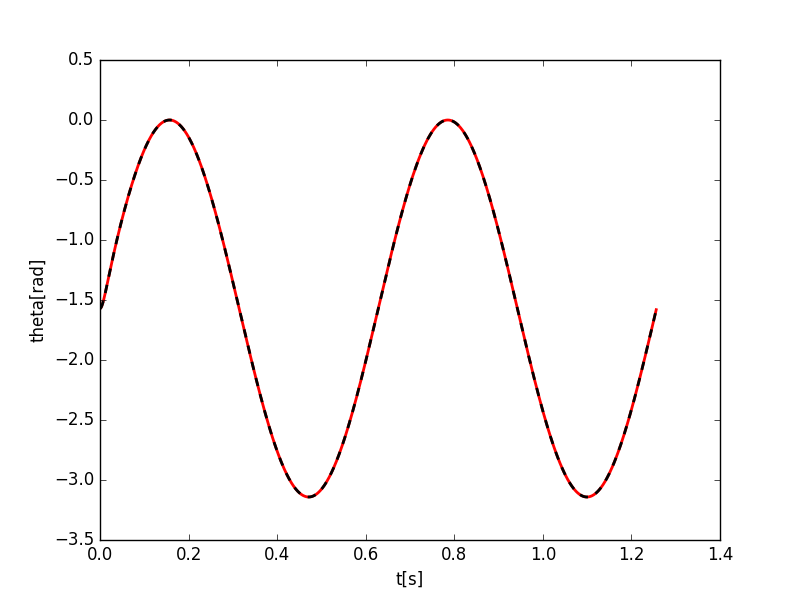
\includegraphics[scale=0.45]{Python/theta.png}
    \end{figure}
\end{frame}

\begin{frame}{Simula\c{c}\~oes}
	\begin{figure}[!h]
        \centering
        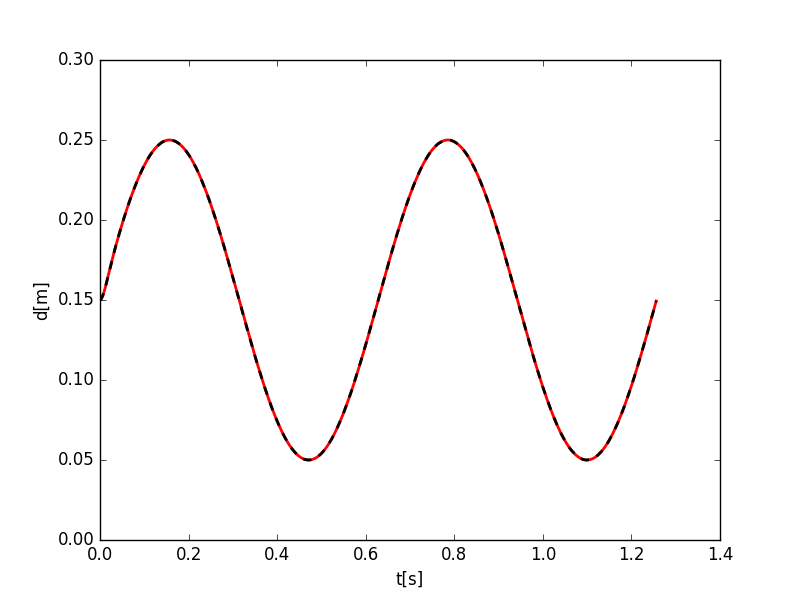
\includegraphics[scale=0.45]{Python/d.png}
    \end{figure}
\end{frame}

\begin{frame}{Simula\c{c}\~oes}
	\begin{figure}[!h]
        \centering
        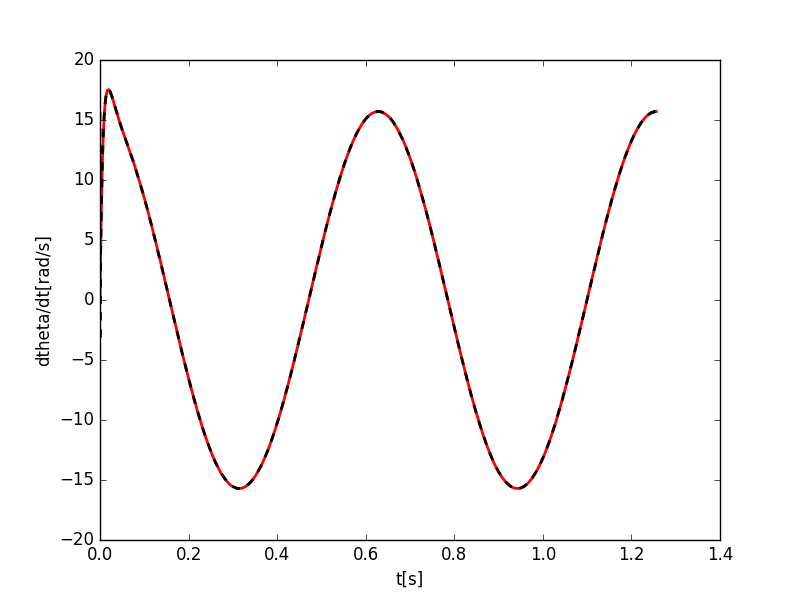
\includegraphics[scale=0.45]{Python/dtheta.png}
    \end{figure}
\end{frame}

\begin{frame}{Simula\c{c}\~oes}
	\begin{figure}[!h]
        \centering
        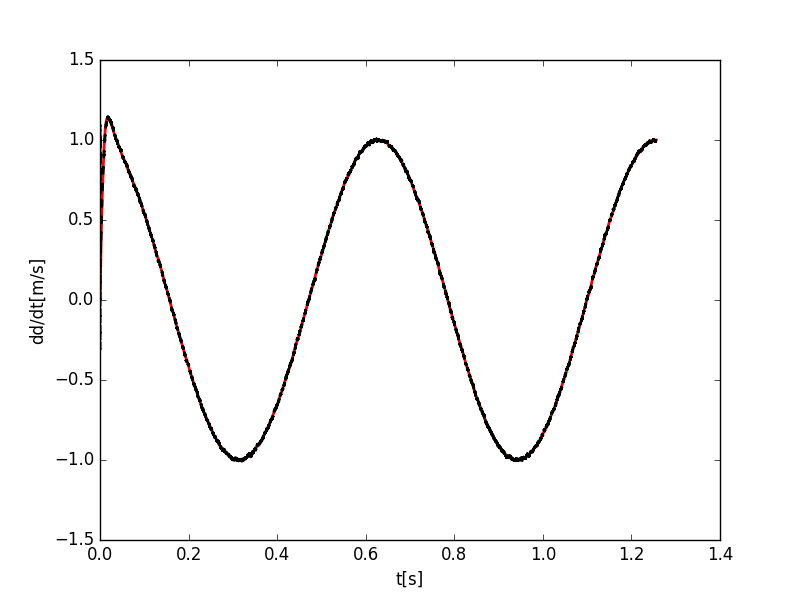
\includegraphics[scale=0.45]{Python/dd.png}
    \end{figure}
\end{frame}

\begin{frame}{Simula\c{c}\~oes}
	\begin{figure}[!h]
        \centering
        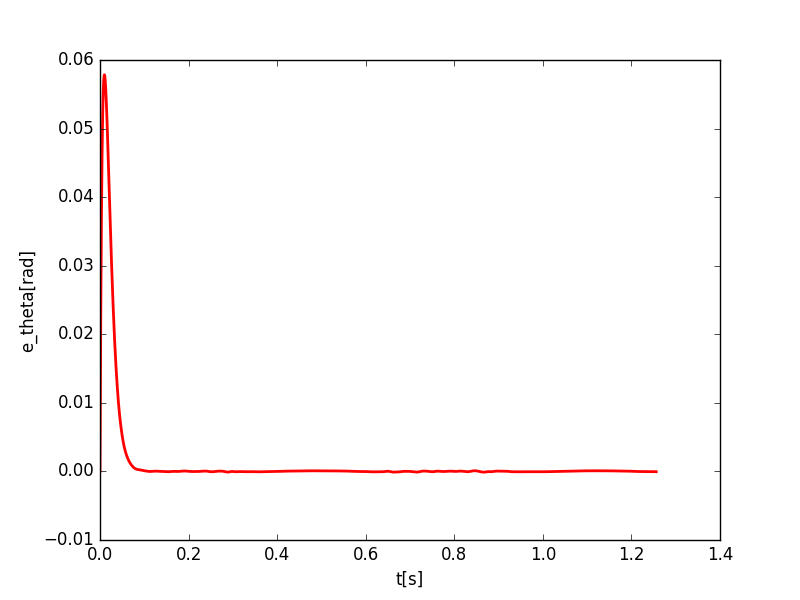
\includegraphics[scale=0.45]{Python/e_theta.png}
    \end{figure}
\end{frame}

\begin{frame}{Simula\c{c}\~oes}
	\begin{figure}[!h]
        \centering
        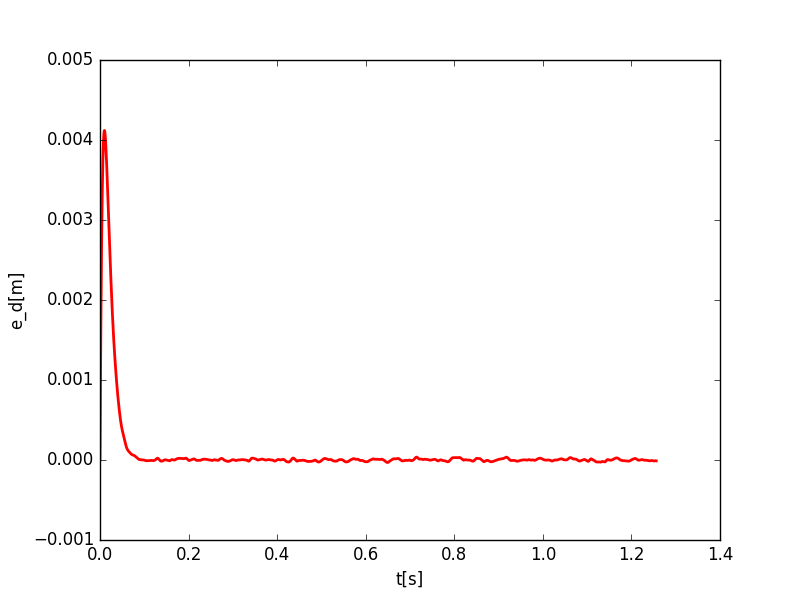
\includegraphics[scale=0.45]{Python/e_d.png}
    \end{figure}
\end{frame}

%\begin{frame}{Conclus\~oes parciais}
%	\begin{block}{}
%		\begin{itemize}
%			\pause
%			\item[$\bullet$] \'E fundamental a utiliza\c{c}\~ao linguagens de alta efici\^encia computacional para realizar  simula\c{c}\~oes din\^amicas de modelos completos de mecanismos complexos
%			\pause
%			\item[$\bullet$] \'E poss\'ivel obter alto desempenho no controle mecanismos paralelos em altas velocidades/acelera\c{c}\~oes utilizando t\'ecnicas de controle n\~ao linear robusto, mesmo com altos n\'iveis de incertezas param\'etricas
%		\end{itemize}
%	\end{block}
%\end{frame}

%-----------------------------------------------------------------------------------------------------------------------------------

\end{document}